\documentclass[border=6pt]{standalone}
\usepackage{amsmath}
\usepackage{amssymb}
\usepackage{tikz}
\usepackage{xcolor}
\usetikzlibrary{arrows.meta,calc,positioning,shapes.geometric}
\begin{document}
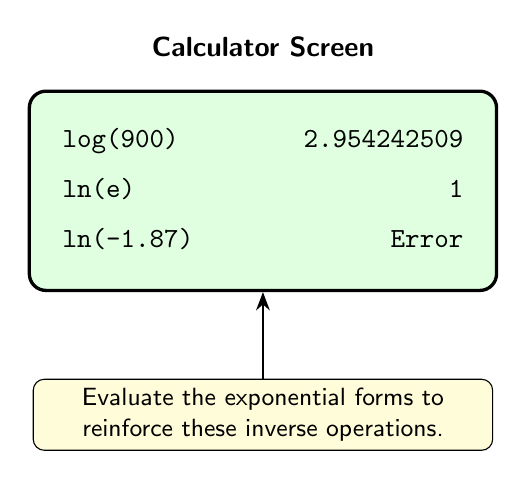
\begin{tikzpicture}[font=\ttfamily]
  % calculator screen
  \node[draw, very thick, rounded corners=6pt, fill=green!12, inner sep=12pt] (screen) at (0,0) {
    \begin{tabular}{@{}l@{\hspace{1.4cm}}r@{}}
      log(900)  & 2.954242509 \\[6pt]
      ln(e)     & 1 \\[6pt]
      ln(-1.87) & Error \\
    \end{tabular}
  };
  \node[font=\sffamily\bfseries, above=0.3cm of screen] {Calculator Screen};

  % callout
  \node[draw, rounded corners=4pt, fill=yellow!15, text width=5.6cm, align=center,
        font=\sffamily\small, below=1.1cm of screen] (callout)
        {Evaluate the exponential forms to reinforce these inverse operations.};
  \draw[-Stealth, thick] (callout.north) -- (screen.south);
\end{tikzpicture}
\end{document}
